\documentclass[tikz,border=2pt]{standalone}
\usepackage{amsmath}
\usepackage{pgfplots}
\pgfplotsset{compat=1.18}
\usetikzlibrary{arrows.meta}
\begin{document}
% Contribution game, low-cost type, when the other player's low type contributes: C gives 3/4,
% D gives q. C is optimal iff q <= 3/4; at q = 1/2 the gap is 3/4 > 1/2.
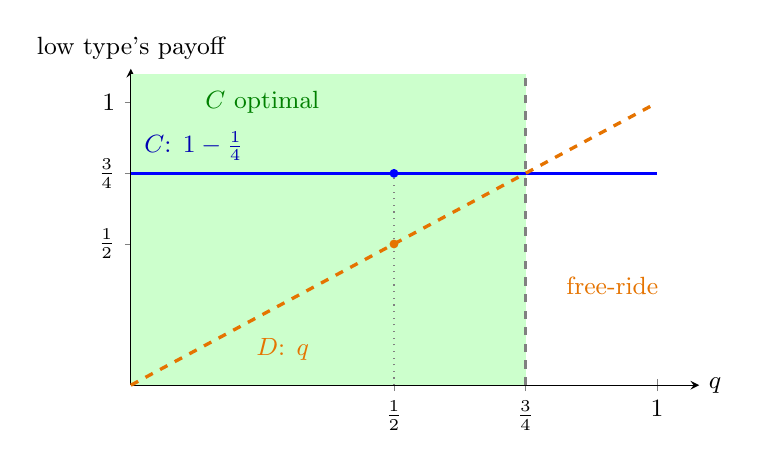
\begin{tikzpicture}[font=\small, >={Latex[length=2mm]}]
  \begin{axis}[
    axis lines=left,
    xmin=0, xmax=1.08, ymin=0, ymax=1.12,
    xtick={0.5,0.75,1}, xticklabels={$\tfrac12$,$\tfrac34$,$1$},
    ytick={0.5,0.75,1}, yticklabels={$\tfrac12$,$\tfrac34$,$1$},
    xlabel={$q$}, ylabel={low type's payoff},
    xlabel style={at={(axis description cs:1,0)}, anchor=west},
    ylabel style={at={(axis description cs:0,1)}, anchor=south, rotate=-90},
    tick label style={font=\small},
    samples=2, clip=false,
    width=8.8cm, height=5.6cm]
    \fill[green!20] (axis cs:0,0) rectangle (axis cs:0.75,1.1);
    \node[green!50!black] at (axis cs:0.25,1.0) {$C$ optimal};
    \node[orange!90!black] at (axis cs:0.915,0.35) {free-ride};
    \draw[gray, dashed, thick] (axis cs:0.75,0) -- (axis cs:0.75,1.1);
    \addplot[blue, very thick, domain=0:1] {0.75};
    \addplot[orange!90!black, very thick, dashed, domain=0:1] {x};
    \node[blue!70!black, anchor=south] at (axis cs:0.12,0.76) {$C$: $1-\tfrac14$};
    \node[orange!90!black, anchor=north west] at (axis cs:0.22,0.2) {$D$: $q$};
    \draw[gray, thin, dotted] (axis cs:0.5,0) -- (axis cs:0.5,0.75);
    \fill[blue] (axis cs:0.5,0.75) circle (1.6pt);
    \fill[orange!90!black] (axis cs:0.5,0.5) circle (1.6pt);
  \end{axis}
\end{tikzpicture}
\end{document}
